\documentclass[a4paper,12pt]{report}
\setcounter{tocdepth}{3}

\usepackage{alltt, fancyvrb, url}
\usepackage{graphicx}
\usepackage[utf8]{inputenc}
\usepackage{float}
\usepackage{hyperref}

% Questo commentalo se vuoi scrivere in inglese.
% \usepackage[italian]{babel}

\usepackage[italian]{cleveref}

\title{Relazione Progetto OOP\\``Dimension Holiday''}

\author{Lorenzo Prati, Elvis Perlika\\ Emanuele Dajko, Alessandra Versari}
\date{\today}


\begin{document}

\maketitle

\tableofcontents

\chapter{Analisi}

\section{Requisiti}

Il gruppo si pone l'obbiettivo di realizzare un videogioco roguelike \textit{Dimension Holiday} vagamente ispirato a giochi famosi come \textit{Hades} oppure \textit{The Binding of Isaac}. Il giocatore controllera' un personaggio che è stato trasportato in un altro mondo dove dovrà
esplorare un dungeon e affrontare un boss per tornare alla propria
dimensione.

\subsection*{Elementi funzionali}

\begin{itemize}
	\item Per attraversare tutto il dungeon il giocatore dovrà passare da stanza in stanza,
	eliminando tutti i nemici presenti. Per farlo potrà usare la spada o lanciare
	proiettili energetici. Giocatore e nemici hanno delle vite (espresse in cuori) e se il giocatore perde tutti i cuori e' \textit{Game over} e si deve ricominciare da capo
	\item Una volta che avrà ucciso tutti i nemici della stanza corrente
	compariranno dei reward casuali (cuori, monete ecc.) e il portale che
	ti trasporterà nella prossima stanza. 
	\item Dopo un certo numero di stanze, comparirà una stanza shop
	dove sarà possibile effettuare acquisti usando le monete creando una piccola progressione
	\item Il gioco si conclude quando il giocatore sconfigge un nemico speciale chiamato \textit{Boss}
	
\end{itemize}

\subsection*{Elementi non funzionali}

\begin{itemize}
	\item Ci si pone l'obbiettivo di creare un'architettura del software modulare ed espandibile ad aggiunte future, come l'aggiunta di nuovi nemici, mappe e oggetti.
\end{itemize}


\section{Analisi e modello del dominio}
Il giocatore potra' muoversi nelle 4 direzioni su, sinsitra, giu', destra tramite i tasti, rispettivamente, W, A, S, D ed effettuare due tipi di attacchi:
\begin{itemize}
	\item \textit{meele}, ovvero ravvicinato, usando una spada e tramite il tasto sinistro del mouse
	\item dalla distanza, usando un proiettile energetico e tramite il tasto destro del mouse
\end{itemize}
Il gioco dovra' essere in grado di presentare al \texttt{giocatore} una serie di stanze dove affrontare dei \texttt{nemici}. Questi potranno avere diversi comportamenti e diverse tipologie di \texttt{attacco}. Il giocatore dovrà stare attento ad evitare gli attacchi dei nemici per non perdere cuori e allo stesso tempo non entrarci in contatto, cosa che comportera' ulteriore danno.
Saranno presenti degli \texttt{oggetti} raccoglibili (cuori, monete ecc.) che dovranno applicare degli \texttt{effetti} alle entita' con cui entrano in contatto, ad esempio l'incremento della vita oppure l'incremento della valuta posseduta dal giocatore. 
Lo shop sara' gestito \textit{in game}, nel senso che non comparirà un'interfaccia grafica che permettera' al giocatore di scegliere i potenziamenti, ma il giocatore dovra' interagire dinamicamente con degli oggetti presenti nella mappa per acquistarli.
Anche gli attacchi applicheranno degli effetti con le entita' con cui entrano in contatto, come ad esempio la perdita di cuori.
Il \texttt{mondo} di gioco (\textit{dungeon}) sara' composto di una serie di stanze. Tramite l'interazione con un oggetto portale, il giocatore sara' trasportato alla stanza successiva senza possibilità di tornare indietro. All'interno delle stanze sono presenti dei muri, che bloccano il passaggio al giocatore. Esistono tre tipi di stanze: normale, shop, boss. Nella stanza normale compariranno dei nemici, in numero e tipo variabile in base al momento della partita, nella stanza shop invece compariranno gli oggetti rappresentati i potenziamenti acquistabili, e nella stanza boss comparirà solo il nemico boss.
Le stanze normali saranno intercambiate randomicamente tra un pool prescelto di mappe create a mano, mentre le stanze shop e boss saranno uniche.

La difficoltà sara' gestita in modo tale che proseguendo nel dungeon risulti piu' difficile il gioco, ad esempio facendo comparire piu' nemici nelle stanze oppure nemici piu' forti. Questo aumento della difficoltà sara' compensato dai potenziamenti che il giocatore potra' acquistare nello shop, che comparira' dopo un numero costante di stanze normali superate. 

Una delle maggiori difficoltà consistera' nella creazione di un architettura che permetta la gestione sia di diversi tipi di nemici (zombie, shooter, boss ecc.), ognuno con un proprio comportamento, sia di diversi attacchi utilizzabili sia dal giocatore che dai nemici (proiettili, attacchi meele). Inoltre, si cerchera' di realizzare un sistema di combattimento \textit{real-time} quanto piu' possibile fluido e responsivo e un'alternanza di mappe e generazione dei nemici in modo tale da far sembrare ogni partita diversa.

Dato il monte ore previsto, si rimanda al futuro una gestione accurata delle performance del gioco.




\chapter{Design}


\section{Architettura}
Abbiamo deciso di utilizzare per il modello logico del gioco e per la logica di controllo una versione semplificata del pattern Entity-Component-System (ECS) mantenendo la parte grafica separata.
Questo pattern si basa come da definizione su tre parti fondamentali, che interconnesse permettono una buona suddivisione delle responsabilita', un alto riuso e un alto grado di composizione (composition over inheritance).



Di seguito spieghiamo le varie parti della nostra architettura:
\begin{itemize}
	\item Components: sono oggetti utili a mantenere dei dati che descrivono un certo aspetto del modello di gioco (ad esempio la posizione sul piano, il movimento, il corpo ecc.). 
	\item Entity: sono dei raccoglitori di Component. Ogni entita' e' descritta dai suoi componenti che permettono alla stessa di distinguerla dalle altre entita'. Ad esempio, diverse entita' presenti in gioco nello stesso momento potrebbero contenere un PositionComponent, un MovementComponent, un BodyComponent, un HealthComponent e altri, che ne descrivono le proprieta' comuni. Tramite l'aggiunta di AIComponent o di un PlayerComponent, solo per citarne alcuni, e' possibile distinguere i nemici dal giocatore. 
	\item Systems: sono la parte dell'architettura che si occupa di operare sulle entita', modificandone i componenti e quindi svolgendo la maggior parte della logica del gioco. L'esecuzione sequenziale di vari sistemi, ciascuno che scorre le entita' e opera su un determinato set di componenti, permette il funzionamento del gioco. Ad esempio, il MovementSystem opera esclusivamente sulle entita' che contengono il MovementComponent e si occupa di muovere tutte le entita'; mentre il CheckHealthSystem si occupa di prendere tutte le entita' che hanno un HealthComponent e di rimuovere quelle che hanno esaurito le vite. E' quindi sufficiente, per inserire nel gioco una nuova meccanica, costruire nuovi componenti che definiscano nuove proprieta' e un nuovo sistema che operi su di essi senza il bisogno di andare a modificare i sistemi o i componenti precedentemente creati.
	\item Engine e World: queste sono le classi che controllano effettivamente lo svolgersi del gioco. Engine si occupa di gestire il game loop, mentre il World contiene al suo interno le entita' di gioco, schedula i system e passa alla View le informazioni necessarie.
	\item View: e' gestita in modo indipendente dal resto dell'architettura e si occupa solamente di disegnare lo stato del modello di gioco. Inoltre, gestisce diverse schermate, si occupa di disegnare l'interfaccia grafica e di registrare gli input da mouse e tastiera.
\end{itemize}

\pagebreak

\section{Design dettagliato}

\subsection{Lorenzo Prati}

Seguendo un approccio bottom-up, di seguito spiego prima il funzionamento della base del \textit{pattern entity-component-system} (\textit{ecs}), per poi passare alla descrizione delle classi fondamentali su cui si poggia il funzionamento dell'applicazione, come Engine e World, e infine dedicarmi ai sistemi e componenti specifici da me realizzati.

\subsubsection{Entity e Component}

\begin{figure}[h]
	\centering
	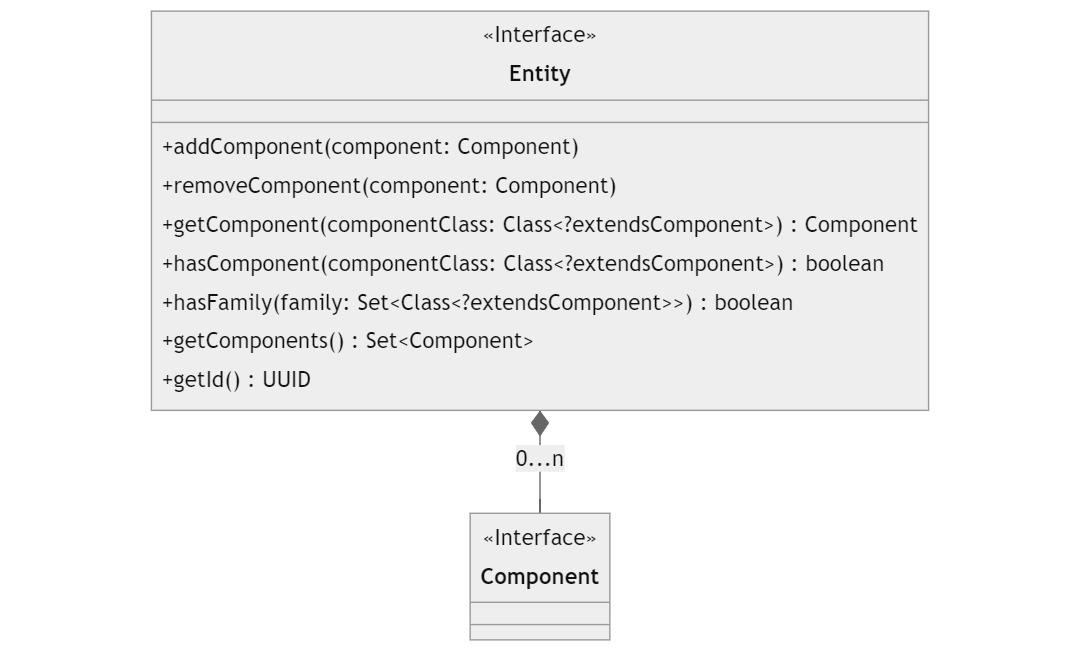
\includegraphics[width=\textwidth]{uml/uml_entity_component.png}
	\caption{Diagramma UML della relazione tra Entity e Component}
	\label{img:badarch}
\end{figure}

\paragraph{Problema}
Modellare il concetto di \textit{entity'} nel contesto del \textit{pattern ecs}. Ogni entita' deve fare riferimento a dei \textit{component} ma non avere una propria logica di comportamento. I componenti devono contenere il piu' possibile solo \textit{dati}. Le entita' devono essere interrogabili sui loro componenti, supportare l'inserimento e la rimozione di componenti, e restituire i componenti richiesti. eventualmente. Nel dominio del gioco, le entita' sono, ad esempio, il giocatore, i nemici, gli oggetti, ma anche gli attacchi.

\paragraph*{Soluzione}
Differentemente dall'approccio classico utilizzato per il \textit{pattern ecs}, che consiste nel rappresentare il concetto di entita' come \textit{id} numerici (interi di fatto) attraverso i quali identificare i vari component, ho scelto di usare un approccio piu' semplice e piu' \textit{object-oriented}, oggetto del corso, realizzando le entita' come classi di tipo \texttt{Entity} contenenti un insieme di \texttt{Component}. Ciascuna entita' possiede comunque un \textit{id} ma questo e' usato in minima parte e solo per esigenze di gestione che esulano da questo paragrafo e che spieghero' in seguito. 
Il vantaggio di questo approccio \textit{oop} e' sicuramente nella semplicita' di gestione; infatti liste di entita', ciascuna con relativo insieme di componenti, sono facilmente iterabili e manipolabili all'occorrenza. Di contro, un approccio piu' a basso livello che favorisca l'uso massiccio di \textit{id} e array di componenti avrebbe permesso un notevole incremento delle performance che pero' e' fuori dallo scopo del progetto.

Quindi, l'interfaccia \texttt{Component} non ha metodi, e serve a essere implementata da tutti i componenti del gioco.
L'interfaccia \texttt{Entity}, invece, contiene tutti i metodi fondamentali per manipolare i componenti contenuti in quell'entita', come ad esempio l'aggiunta e la rimozione, e l'ottenimento di uno specifico componente. Tramite il metodo \texttt{hasFamily} e' possibile interrogare l'entita' sul possesso di un insieme di \texttt{Component} specifici, cosa che risultera' molto utile per i \textit{system}.

Su queste semplici interfacce si basa l'intera struttura del \textit{pattern entity-component-system}, o meglio della parte \textit{entity-component} che rappresenta in questo caso il modello del gioco (lo \textit{stato} e i \textit{dati}), mentre la \textit{logica di controllo} e' affidata ai \textit{system}.

Infine, ho realizzato una classe \texttt{EntityBuilder} che, tramite l'uso del \textit{builder pattern}, consente la creazione di entita' in modo dichiarativo semplicemente tramite l'aggiunta sequenziale di \texttt{Component} su cui si basano tutte le factory presenti nel progetto. Per creare nuove entita' e' quindi sufficiente aggiungere componenti tramite l'\texttt{EntityBuilder} e modificando i parametri di creazione di questi componenti oppure creandone di nuovi, e' di fatti possibile creare molto velocemente nemici, oggetti e attacchi nuovi e dalle caratteristiche diverse. (vedi factories)

\subsubsection{System}

\begin{figure}[h]
	\centering
	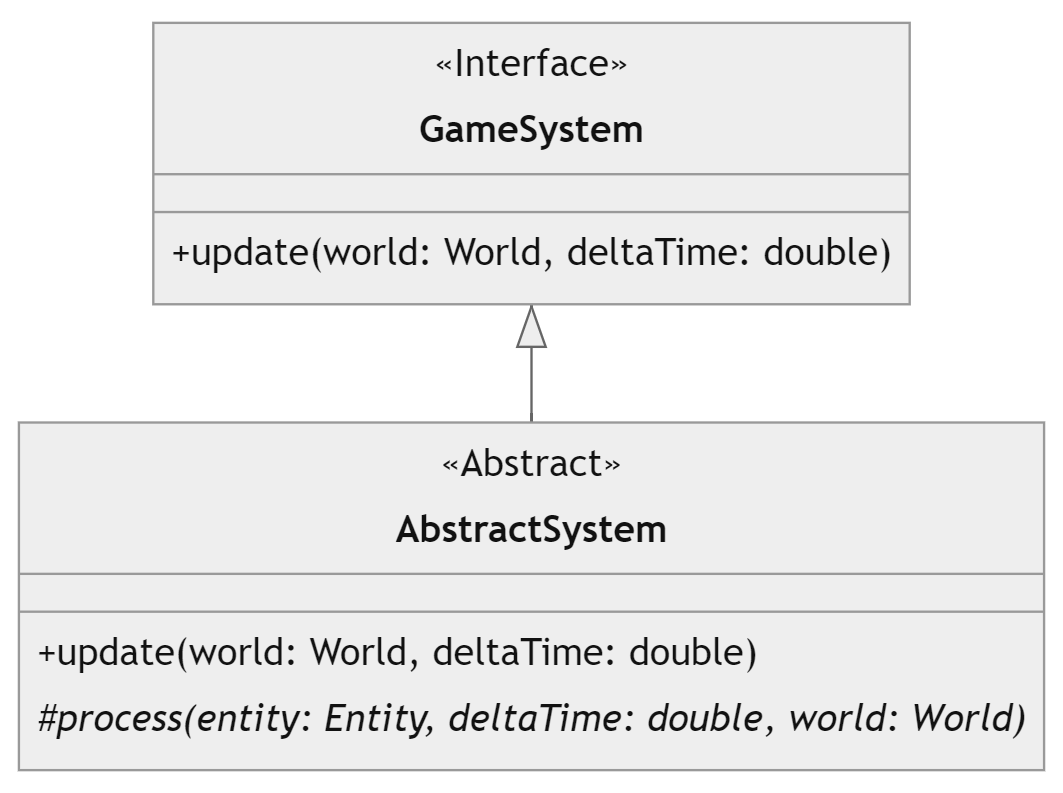
\includegraphics[width=\textwidth]{uml/uml_system.png}
	\caption{Diagramma UML dei \textit{system}} 
\end{figure}

\paragraph{Problema}
Le entita' e i componenti non definiscono logica di comportamento propria, quindi e' necessario che vengano manipolati dai \textit{system}. I sistemi devono essere divisi per specifico compito e ognuno deve essere in grado di riconoscere su quali entita' e' in grado di operare. Ad esempio, devono essere realizzati dei sistemi in grado di muovere le entita', gestire le loro collisioni, rimuoverle dal mondo di gioco quando necessario ecc.

\paragraph[]{Soluzione}
Ho realizzato un'interfaccia \texttt{GameSystem} che modella un generico \textit{system}. Il metodo esposto e' \texttt{update} e si occupa di far eseguire la logica del sistema. Visto che ogni \textit{system} deve essere in grado di operare solo su certe entita', per garantire il \textit{riuso} ho scelto di realizzare una classe astratta \texttt{AbstractSystem} che all'interno utilizza il \textit{pattern template method} dove il metodo template e' appunto \texttt{update}, che fa i dovuti controlli sulle entita' e poi richiama il metodo astratto e protetto \texttt{process} solo sulle entita' che hanno i componenti richiesti. In questo modo, ogni classe che estende \texttt{AbstractSystem} deve solamente occuparsi di definire tramite costruttore l'insieme di \texttt{Component} su cui vuole operare e poi implementare il metodo \texttt{process} che andra' ad operare solo su \texttt{Entity} che hanno i componenti precedentemente richiesti.

I \textit{system} sono in grado, avendo nel loro metodo \texttt{process} un riferimento al \texttt{World} di notificare, come spieghero' meglio in seguito, degli eventi; ma e' anche possibile un metodo di \textit{signaling} tra \textit{system} diversi. Questo e' possibile attaccando, in seguito al verificarsi di una determinata situazione, un componente \textit{informativo} all'entita' che si sta processando in modo tale da permettere a successivi \textit{system} di cercare entita' con quel componente \textit{informativo} e gestire la cosa adeguatamente.

\subsubsection{Engine}

\begin{figure}[h]
	\centering
	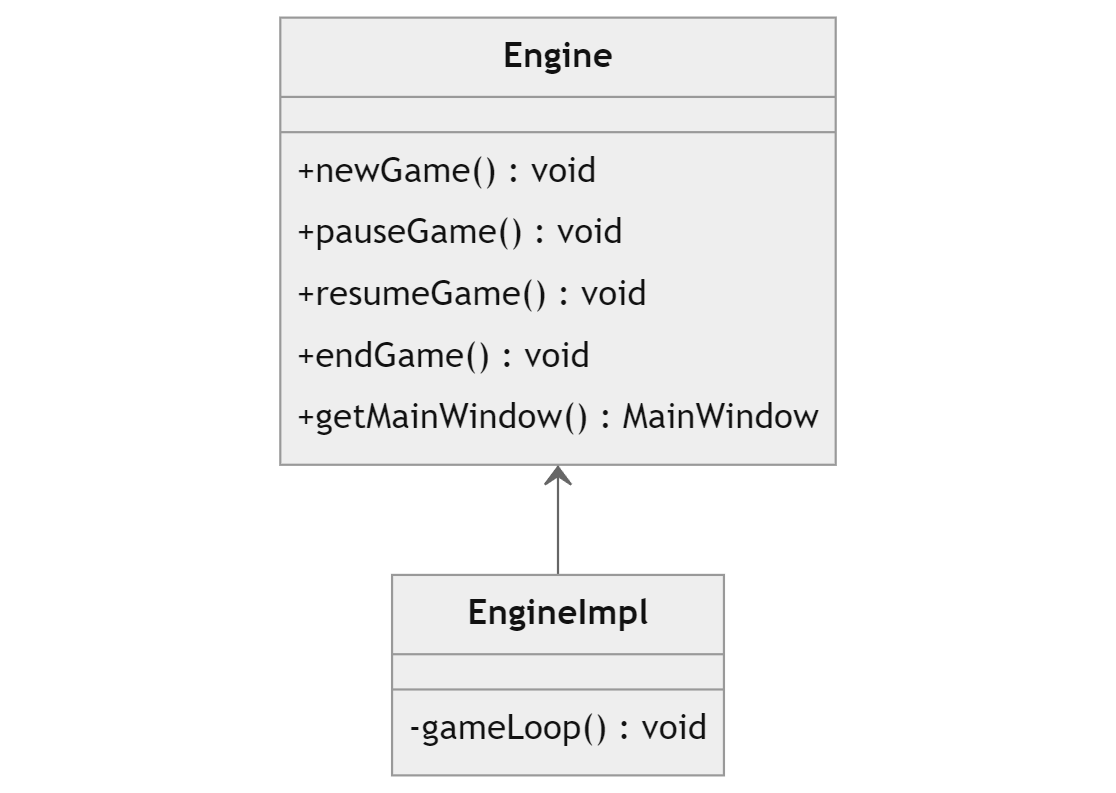
\includegraphics[width=\textwidth]{uml/uml_engine.png}
	\caption{Diagramma UML dell'Engine}
	\label{img:badarch}
\end{figure}

\paragraph*{Problema}
Realizzare una classe che permetta lo svolgimento effettivo del main loop del gioco, attraverso il quale scandire gli update del modello logico e della rappresentazione grafica, e che contenga tutti gli elementi per mantenere attiva l'applicazione. All'occorrenza, deve anche essere possibile mettere in pausa il gioco e riprenderlo. Deve essere inoltre gestita la fine del gioco.

\paragraph*{Soluzione} La soluzione e' ricaduta sulla creazione di un'interfaccia \texttt{Engine} con relativa implementazione \texttt{EngineImpl}. Questa classe fa uso del \textit{pattern game loop}, realizzato in un metodo privato e vengono esposti dall'interfaccia i metodi necessari alle altre classi (ad esempio le schermate della View) per controllare il loop. E' quindi possibile metterlo in pausa, riprenderlo e arrestarlo. Essendo questa classe la prima che viene creata al lancio dell'applicazione, essa si occupa anche internamente di creare il modello logico e la view.

\subsubsection{World}

\begin{figure}[h]
	\centering
	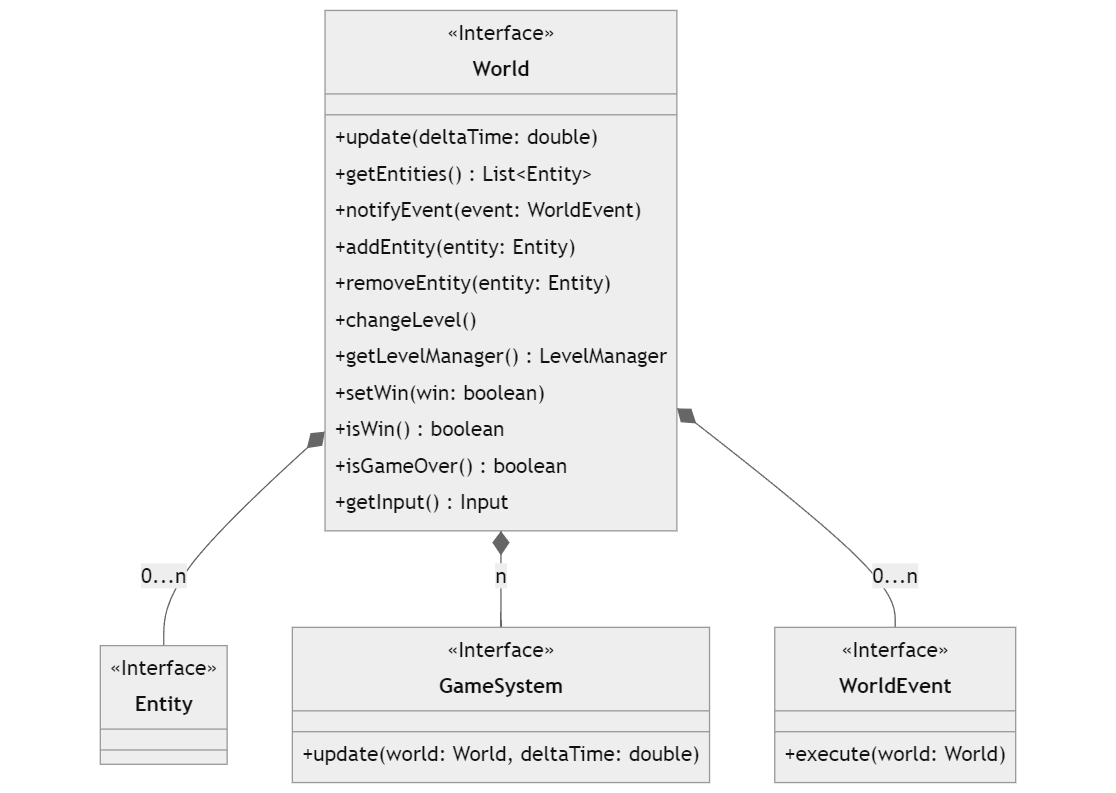
\includegraphics[width=\textwidth]{uml/uml_world.png}
	\caption{Diagramma UML del World}
	\label{img:badarch}
\end{figure}

\paragraph*{Problema}
Occorre contenere e mantenere le \texttt{Entity}, e comandare la logica che opera su di esse, cioe' i \textit{system}. Allo stesso tempo, e' necessario passare alla View le informazioni necessarie affinche' possa disegnare sia le entita' che la mappa di gioco. 

\paragraph*{Soluzione}
Ho scelto di unire in un'unica classe la funzione di contenere le entita' e i sistemi, e la rappresentazione grafica del mondo di gioco (\texttt{Scene}), quindi ho realizzato l'interfaccia \texttt{World} con la relativa implementazone \texttt{WorldImpl}. Ho optato per questa scelta di nome nonostante la funzione della classe sia piu' comparabile a quella di un classico \textit{Controller} del pattern MVC poiche' e' utilizzato spesso nel contesto del \textit{pattern ecs}.

L'interfaccia \texttt{World} espone i metodi necessari al controllo del gioco vero e proprio, come ad esempio il metodo \texttt{update}, che viene chiamato ad ogni ciclo del \textit{game loop} in esecuzione sull'\texttt{Engine}. Questo e' il metodo principale della classe, perche' si occupa di:

\begin{itemize}
	\item eseguire tutti i \texttt{GameSystem} 
	\item eseguire tutti gli eventi in coda nel \texttt{World}
	\item comandare alla scena di disegnare
\end{itemize}

Ho scelto di memorizzare e gestire i \texttt{GameSystem} direttamente in una lista dentro il \texttt{World} per semplicita' quando di fatti l'ordine con cui essi vengono memorizzati nella lista e quindi eseguiti ad ogni ciclo di \textit{update} potrebbe essere gestito da uno \textit{strategy pattern} ed essere modificabile in futuro con un'altra implementazione; tuttavia ho scelto di semplificare l'approccio perche' in ogni caso non viene gestita in nessun modo l'abilitazione/disabilitazione di sistemi a run-time (come e' comune nel \textit{pattern ecs}) e in generale in un gioco semplice come il nostro i pochi sistemi presenti devono eseguire strettamente uno dopo l'altro in un certo ordine preciso che di fatti lascia spazio a poche variazioni. Per quest'ultimo motivo, la gestione dei sistemi e' fissa e non modificabile, e per questo l'inizializzazione dei \texttt{System} e' gestita internamente al \texttt{World} e non e' visibile o modificabile dall'esterno.

Poi il \texttt{World} espone i metodi per la gestione delle \texttt{Entity}, cioe' che permettono di aggiungere e rimuovere \texttt{Entity}, oppure di avere una copia delle entita' presenti in gioco.

Gli eventi sono rappresentati tramite l'interfaccia \texttt{WorldEvent} e sono gestiti in modo asincrono. Durante la loro esecuzione, i vari \textit{system} possono notificare il \texttt{World} di uno specifico evento, che verra' messo in una coda ed eseguito solo dopo che tutti i \texttt{System} hanno finito la loro esecuzione. In questo modo si evita il verificarsi di comportamenti anomali dovuti all'immissione di \texttt{Entity} nel \texttt{World} nel mezzo dell'esecuzione dei \textit{system} durante la quale, d'altra parte, e' risultato comodo sia immettere che rimuovere le \texttt{Entity} tramite eventi dedicati, in modo da reagire all'aggiunta/eliminazione di una specifica entita' (ad esempio per il \textit{game over}). Mi sono occupato io di implementare tutti gli eventi, che saranno pero' lanciati anche dai \textit{system} realizzati dai miei colleghi:
\begin{itemize}
	\item \texttt{AddEntityEvent} aggiunge l'entita' passata come parametro al \texttt{World}
	\item \texttt{RemoveEntityEvent} rimuove dal \texttt{World} l'entita' passata come parametro, in questo caso identificata tramite \textit{id}. Nel caso si trattasse dell'entita' che rappresenta il giocatore o il boss, viene notificato il \texttt{World} rispettivamente della sconfitta e della vittoria tramite il metodo \texttt{setWin(boolean win)}
	\item ChangeLevelEvent chiama il metodo \texttt{changeLevel()} del \texttt{World}, che procede a gestire il cambio di livello aggiornando le entita' con quelle generate dal \texttt{LevelManager} per il nuovo livello e passando alla \texttt{Scene} anche la nuova mappa.
\end{itemize}

Il \texttt{World} espone anche un metodo per ottenere la classe con la quale i \texttt{System} possono sfruttare l'input dell'utente, che spieghero' piu' nel dettaglio descrivendo il funzionamento del giocatore.

Infine, sono presenti vari metodi che servono a interrogare il \texttt{World} sullo stato della partita
(\texttt{isGameOver()}) e il risultato della partita (\texttt{isWin()}), utili soprattutto all'\texttt{Engine} che deve sapere quando arrestare il \textit{game loop} e gestire la fine del gioco.

\subsubsection{Movimento e Posizione}

\begin{figure}[h]
	\centering
	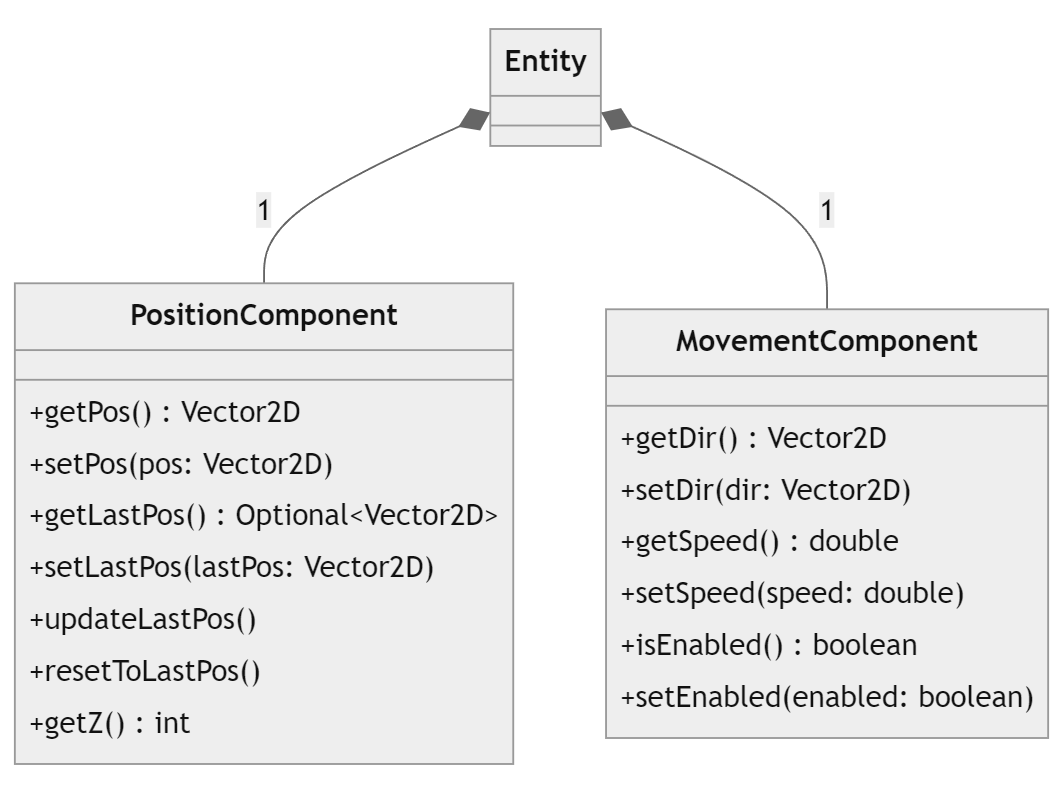
\includegraphics[width=\textwidth]{uml/uml_pos_mov.png}
	\caption{Diagramma UML dei componenti della posizone e del movimento}
\end{figure}

\paragraph{Problema}
Tutte le entita' di gioco occupano una posizione nella mappa di gioco, che a livello di modello possiamo rappresentare come un piano 2d. Mentre alcune entita' mantengono la loro posizione invariata nel tempo (come gli item), altre (come i nemici e il giocatore) variano la posizione nel tempo muovendosi in diverse direzioni secondo le logiche dell'intelligenza artificiale o un input dell'utente.

\paragraph{Soluzione}
Ho realizzato una classe \texttt{PositionComponent} che ovviamente implementa l'interfaccia \texttt{Component} e memorizza le coordinate della posizione di un'entita' in quel momento. Inoltre, al suo interno viene memorizzata anche la posizione precedente a quella corrente, poiche' sara' utile nel momento di gestire le collisioni. La posizione viene quindi memorizzata come dato all'interno del componente, cosi' da poter attaccare ad ogni entita' (tutte di fatto) che hanno una posizione nella mappa un \texttt{PositionComponent}, massimizzando il \textit{riuso di codice}. 

Analogamente, per rappresentare il movimento ho creato un componente \texttt{MovementComponent}, che memorizza la direzione in cui il movimento deve essere compiuto, tramite un vettore 2d. Inoltre, viene qui memorizzata anche la velocita' con la quale l'entita' dovra' compiere il movimento. Il movimento puo' anche essere abilitato/disabilitato. La scelta di gestire il movimento tramite vettori, nonostante le entita' di gioco si muovano quasi tutte soltanto nelle 4 direzioni, permette in futuro anche la facile implementazione del movimento nelle 8 direzioni, o comunque una sua gestione libera.

Una volta definiti questi componenti di base, e' possibile gestire il movimento di tutte le entita' tramite un \textit{system}. Il \texttt{MovementSystem} si occupa infatti di filtrare le entita' che hanno un componente \texttt{MovementComponent}, che significa che \textit{posseggono la capacita' di muoversi e hanno i dati necessari affinche' possano essere mosse}, e si occupa di verificare per ciascuna di queste entita' se il movimento e' abilitato (vedi sopra) e nel caso aggiornare il \texttt{PositionComponent} con la nuova posizione risultante dal calcolo del movimento espresso nel \texttt{MovementComponent} applicato alla vecchia posizione. L'esecuzione di questo \textit{system} ad ogni ciclo del \textit{game loop}, permette di muovere tutte le entita' che \textit{possono farlo} previo precedente settaggio della direzione in cui l'entita' intende muoversi.

\subsubsection{Collisioni e fisica}

\begin{figure}[h]
	\centering
	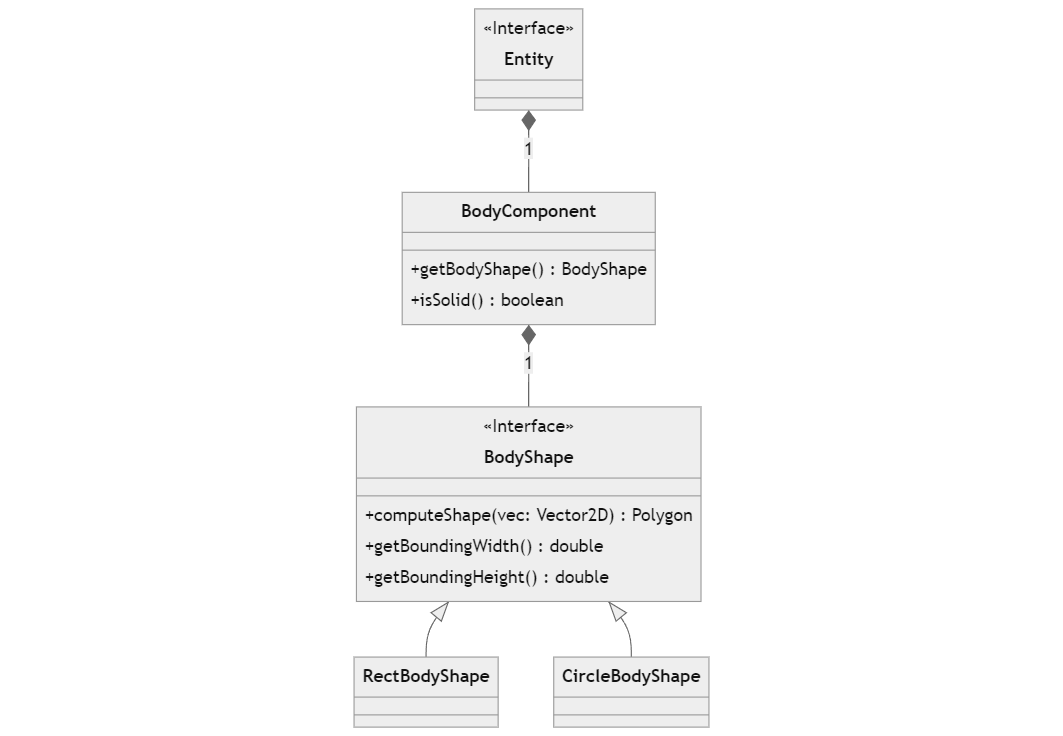
\includegraphics[width=\textwidth]{uml/uml_body.png}
	\caption{Diagramma UML del componente del corpo e delle shape}
\end{figure}

\paragraph{Problema}
Alcune entita' hanno corpi \textit{solidi} e devono comportarsi come tali nelle loro azioni di movimento. Inoltre e' necessario registrare quando entita' di qualunque tipo collidono con altre entita', al fine di poterne gestire le conseguenze.

\paragraph{Soluzione}
Ho realizzato una classe \texttt{BodyComponent} che modella il \textit{corpo} di un'entita', definendone proprieta' come la \texttt{BodyShape}, ovvero la forma geometrica che il suo corpo occupa nello spazio, e la solidita'.
(espressa da un booleano). 

Il \texttt{CollisionSystem} si occupa di processare le entita' che hanno un \texttt{BodyComponent}. Per ciascuna di queste entita', viene controllata la collisione con \textit{tutte} le altre entita' presenti nel gioco. Se viene rilevata una collisione, calcolata estrendo dai rispettivi \texttt{BodyComponent} le body shape e controllandone l'intersezioni in date coordinate, allora viene \textit{registrata} la collisione attaccando all'entita' che il system sta processando in quel momento un \texttt{CollisionComponent}, un semplice componente che mantiene i dati sulle collisioni avvenute. In particolare, viene aggiunto un \texttt{CollisionComponent} solo nel caso non ce ne sia gia' uno, poiche' altrimenti vengono aggiornate le informazioni di quello gia' presente aggiungendo i dati sulla nuova collisione. Questo e' un esempio, l'unico in realta' realmente presente in questo progetto, di \textit{signaling tra system}. Infatti, i successivi \textit{system} potranno filtrare le entita' che hanno tra i loro componenti anche un \texttt{CollisionComponent} e gestire la collisione in modo appropriato. Su questo meccanismo si basano i sistemi che gestiscono le collisioni fisiche, gli item, il combattimento ecc. poiche' la loro gestione si basa sulla precedente aggiunta di un \texttt{CollisionComponent} da parte del \texttt{CollisionSystem}.

Un \texttt{PhysicsSystem}, che esegue subito dopo il \texttt{CollisionSystem}, processa le entita' che hanno \texttt{BodyCompoenent} e \texttt{CollisionComponent} occupandosi invece della gestione vera e propria della collisione fisica, che pero' nel dominio del gioco si traduce in un semplice reset della posizione. Dato che vengono tenute nel \texttt{PositionComponent} sia la posizione corrente che quella immediatamente passata, solo in caso di collisione tra corpi \textit{solidi} viene ripristinata la posizione precedente.

Menziono qui anche la presenza di un \texttt{ClearCollisionSystem}, un semplice sistema che esegue dopo che hanno eseguito tutti i sistemi che dovevano in qualche modo gestire la reazione a una collisione (filtrando anche per \texttt{CollisionComponent}), rimuovendo tutti i \texttt{CollisionComponent} dalle entita' che ne hanno uno. In questo modo, al successivo loop di update dei system, non vengono lasciate collisioni non gestite.

Per quanto riguarda ingine l'interfaccia \texttt{BodyShape}, essa puo' essere implementata potenzialmente da classi che rappresentano varie forme geometriche. Io ho realizzato una \texttt{RectBodyShape}, che rappresenta la forma geometrica del rettangolo, e una \texttt{CircleBodyShape}, che rappresenta il cerchio. L'interfaccia espone il metodo \texttt{computeShape(Vector2D)} che permette di ricevere il poligono calcolato in base alle coordinate fornite, utile poi al calcolo dell'intersezione con un altro poligono. Qui ho fatto uso di libreria come spiegato meglio nel paragrafo dedicato (riferimento). Inoltre, sono presenti i metodi \texttt{getBoundingWidth} e \texttt{getBoundingHeight} per conoscere il rettangolo che limita il poligono, utili sia alla View che in altri punti del progetto.

\subsubsection{Logica del giocatore e Input}

\begin{figure}[h]
	\centering
	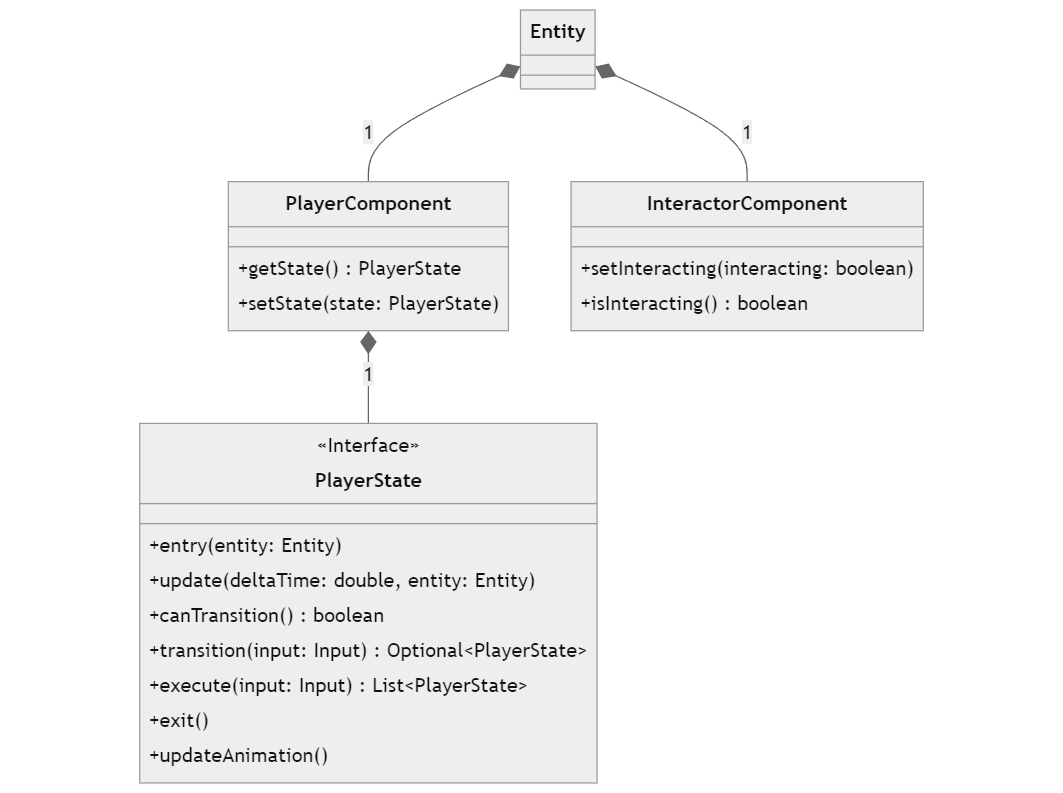
\includegraphics[width=\textwidth]{uml/uml_player.png}
	\caption{Diagramma UML dell'entita' che rappresenta il giocatore e alcuni dei suoi componenti}
\end{figure}

\paragraph{Problema}
L'utente controlla un personaggio in grado di:

\begin{itemize}
	\item muoversi in 4 direzioni (su, giu', destra, sinistra)
	\item attaccare con la spada
	\item sparare un proiettile
	\item caricare una palla di fuoco e spararla rilasciando il tasto
	\item interagire con oggetti
\end{itemize}

Ognuna di queste azioni e' rappresentata a schermo da un'animazione differente. Alcune di queste azioni hanno condizioni per poter essere eseguite, oppure possono essere eseguite solo dopo aver compiuto altre azioni; ma in ogni momento il giocatore esegue solo una di queste azioni.

\paragraph{Soluzione}
Ho risolto il problema utilizzando lo \textit{state pattern} in combinazione con un \texttt{PlayerInputSystem}. Infatti, se abbiamo cercato di rispettare il pattern \textit{ecs} il piu' possibile, specialmente cercando di gestire la logica di comportamento delle entita' interamente nei \textit{system} quando possibile, si e' convenuto che non abbia senso forzarlo su ogni aspetto, percio' in questo e in altri casi parte della logica e' stata spostata fuori dai system cercando di semplificare l'aspetto del \textit{behaviour} presente in alcune implementazioni dell'\textit{ecs}. 

In questo caso, il giocatore e' un entita' come le altre, definita dall'insieme dei suoi componenti. Il componente che lo distingue maggiormente pero' e' il \texttt{PlayerComponent}, che non contiene lui stesso la logica del comportamento del player, ma contiene delle classi che hanno questa logica, cioe' gli \textit{stati} del player (\texttt{PlayerState}). 

Il \texttt{PlayerInputSystem}, che e' il primo \textit{system} a eseguire nel gioco ad ogni loop, processa le entita' che hanno un \texttt{PlayerComponent} (lasciando quindi aperta la possibilita' di gestire piu' giocatori). Per semplicita' di spiegazione, assumiamo che l'entita' che rappresenta il giocatore sia una sola. In questo caso, tale entita' viene processata normalmente dal sistema, che ne gestisce il \textit{cambio di stato} in base all'input dell'utente agendo come parte di una \textit{finite state machine}.

\begin{figure}[h]
	\centering
	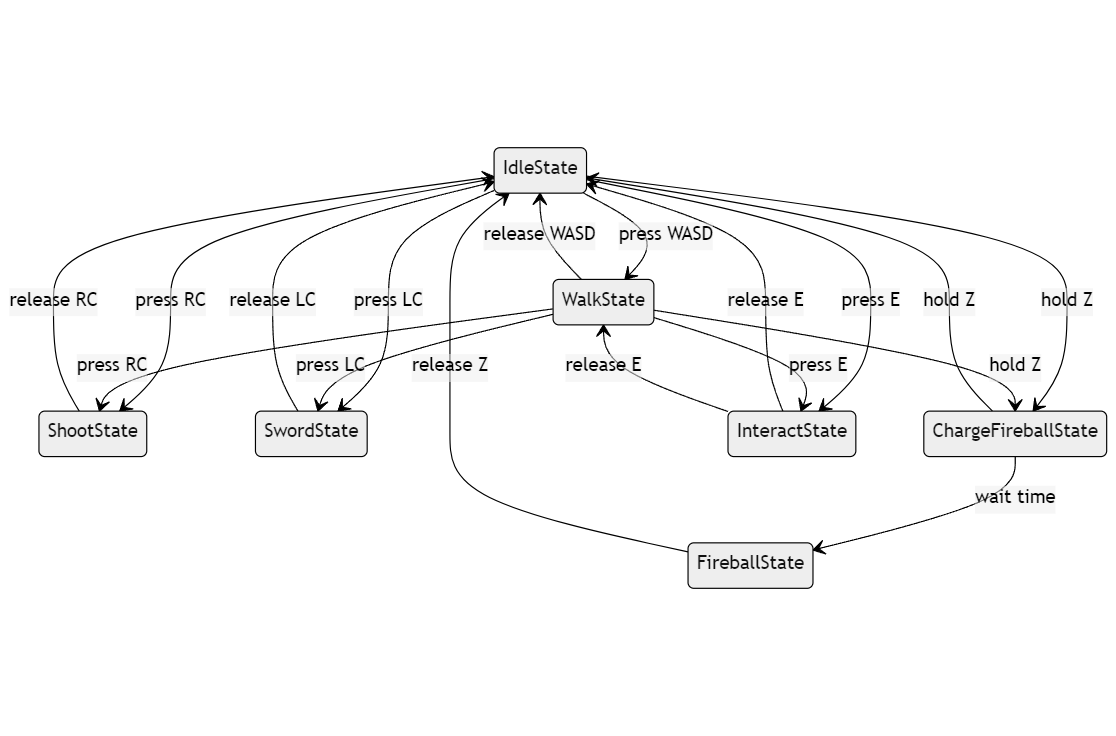
\includegraphics[width=\textwidth]{uml/player_states.png}
	\caption{Diagramma degli stati del player. LC ed RC indicano rispettivamente il tasto sinistro e destro del mouse. Il player puo' trovarsi solo in uno di questi stati alla volta} 
\end{figure}

Il \texttt{PlayerComponent} contiene lo \textit{stato} corrente in ogni momento, quindi viene estratto tale \texttt{PlayerState} e interrogato sulla possibilita' di poter effettuare un cambio di stato in base all'\texttt{Input}; se possibile, quindi, il \texttt{PlayerState} corrente restituisce il prossimo stato calcolato sempre sulla base dell'input e il system procede con la transizione di stato, sostituendo lo stato corrente nel \texttt{PlayerComponent} con il nuovo stato calcolato. Se lo stato corrente puo' transitare, allora viene anche chiamato il metodo \texttt{execute}, che potrebbe generare nuove entita', ad esempio proiettili o attacchi, e queste vengono poi aggiunte al \texttt{World} tramite evento. Il cambio di stato piu' nel dettaglio e' gestito dai metodi \texttt{entry} ed \texttt{exit} che gestiscono rispettivamente le operazioni da effettuare nei due momenti per quello stato. Infine, il system aggiorna l'animazione (vedi spiegazione animazioni). 

Ora analizzo piu' nel dettaglio i vari stati. Ciascuno di essi estende una classe \texttt{AbstractState} che fattorizza alcuni metodi dell'interfaccia \texttt{PlayerState} come \texttt{canTransition()} (che si occupa di controllare che lo stato non sia bloccato in un animazione non cancellabile), \texttt{update(double, Entity)} e altri che sono utili alle sottoclassi come \texttt{setAnimationState(String)}. Inoltre, vengono fortnite delle implementazioni di default dei metodi d'interfaccia \texttt{entry(Entity), \texttt{exit()}} e \texttt{execute(Input)}, overridabili a piacimento dalle sottoclassi per definire comportamenti piu' complessi. Invece, il metodo \texttt{transition(Input)} e' lasciato astratto da implementare per ogni singolo stato poiche' ognuno definisce logiche proprie di transizione verso altri stati, che non descrivo nei dettagli poiche' credo gia' sufficiente esplicate nel diagramma sopra. Infine, ogni stato implementa il metodo \texttt{updateAnimation()} settando una specifica animazione (riferimento alla speigazione delle animazioni).

Di seguito gli stati:
\begin{itemize}
	\item \texttt{IdleState} rappresenta lo stato di \textit{idle}, cioe' in cui il giocatore e' fermo, e si occupa solo di disabilitare il movimento in entrata.
	\item \texttt{WalkState} rappresenta lo stato di camminata, e si occupa di abilitare/disabilitare il movimento in entrata/uscita e di settare la direzione del \texttt{MovementComponent} coerentemente con l'input dell'utente.
	\item \texttt{SwordState} rappresenta lo stato di attacco ravvicinato, 
\end{itemize}

L'interfaccia \texttt{Input} e'ottenibile tramite getter dal \texttt{World} e interrogabile sui tasti premuti dall'utente tramite dei semplici getter; in questo modo i vari stati sono in grado di sapere quali azioni sta attualmente cercando di realizzare l'utente.

Ho realizzato una classe \texttt{InputListener} che, tramite i metodi di Swing, registra l'input da mouse e tastiera e chiama dei setter su un'istanza di \texttt{Input}. Questa istanza viene poi passata al \texttt{World} tramite una copia, garantendo in questo modo al modello di gioco di operare con una classe completamente separata dalla View.

\subsubsection{Schermata vittoria/sconfitta}
Ho realizzato anche una schermata di View, cioe' la schermata di vittoria e sconfitta. Qui, tramite il passaggio di un parametro booleano che indica la vittoria/sconfitta, viene semplicemente visualizzata un'immagine di sfondo e un messagio finale differente.


\subsection{Elvis Perlika}

\subsection{Emanuele Dajko}

\subsection{Alessandra Versari}
\begin{itemize}
	\item Items: Con item si intende un oggetto di gioco che verrà raccolto a seguito del passaggio del player sopra ad esso. Gli item presenti nel nostro gioco sono cuori e monete.
	Ciascun item una volta entrato in contatto con un'entità deve prima verificare che si tratti del player ed effettuare i controlli necessari prima di applicare il proprio “effetto” (cioè la conseguenza/reazione che l'item avrà sull'entità che ha colliso con esso).
	Di seguito le principali caratteristiche degli items presenti nel nostro gioco:
	\begin{itemize}
		\item Gli items “cuore” permetteranno di aumentare la vita corrente del player, ma ciò verrà fatto solo a seguito del controllo sulla vita corrente: l'item verrà raccolto se e solo se la vita corrente è minore della vita massima che il player può avere. Questo tipo di item è disponibile in ogni stanza, escludendo lo Shop.
		\item Gli items “moneta”, anch'essi presenti in ciascun livello (shop escluso), permetteranno di aumentare l'ammontare delle monete raccolte dal player. Questo tipo di item, oltre a verificare che l'entità che ha colliso con esso sia il player, non farà ulteriori controlli. Lo scopo degli items “moneta” è quello di consentire al player, l'acquisto di power up (che tratterò in seguito) all'interno della stanza Shop.
	\end{itemize}
	Per realizzare quanto descritto ho deciso di creare due componenti principali: HealthComponent e CoinPocketComponent, appartenenti alla lista di componenti del player, che permettono di consultare e modificare vita corrente, vita massima e monete raccolte. Tramite i getter e i setter, in questo modo, posso creare gli “effetti” degli item, all'interno dell'ItemFactory. 
	Ogni item è dotato di un componente detto ItemComponent che oltre a rendere riconoscibili gli item, memorizza una Bifunction che corrisponde a quello che fin'ora ho definito “effetto”. La Bifunction in questo caso prende come argomento l'entità che ha colliso con l'item e una lista di component. Nel nostro gioco, al momento, solo il player ha la possibilità di raccogliere items, ma nel caso in cui volessimo rendere questi items raccoglibili anche ai nemici, sarebbe possibile farlo, passando come argomento alla Bifuntion una lista contenente i componenti identificativi di player e nemici (ossia PlayerComponent e AIComponent).
	Inizialmente avevo scelto di creare gli effetti utilizzando il Factory Method perché pensavo potesse rendere più riutilizzabili gli effetti e velocizzarne la creazione, ma il risultato era un insieme di classi Factory, molto simili tra loro e la cui unica differenza era operare su componenti diversi (una factory per gli effetti che modificavano la vita, un'altra per quelli che modificavano l'ammontare delle monete e così via).
	Inoltre siccome gli effetti alla fine sono praticamente solo incrementi e decrementi, mi è sembrato più sensato utilizzare interfacce funzionali e lamba per crearli all'interno della factory. 
	Per quanto riguarda le interfacce funzionali, ho deciso di utilizzare le Bifuction così da poter restituire un boolean che permette di capire se l'effetto è stato applicato o meno e se quindi è necessario rimuovere l'item.

	Nella classe ItemFactory è stato utilizzato il Factory Method.
	\item InteractableObjects: Con interactable objects si intende tutti gli oggetti di gioco che per essere utilizzati necessitano dell'interazione del giocatore. A differenza degli items infatti, la collisione con l'oggetto in questo caso non è sufficiente, è necessario premere in tasto E una volta posizionato il player sull'oggetto.
	Gli oggetti interactable presenti nel nostro gioco sono i power-up e il gate. 
	I power-up sono potenziamenti che il player può acquistare nella stanza shop pagando il loro prezzo. Essi si suddividono in:
	\begin{itemize} 
		\item Power-up vita: permette di aumentare la vita massima del giocare.
		\item Power-up velocità: permette di aumentare la velocità del giocatore.
	\end{itemize}
	Il gate invece è semplicemente il portale che permette di accedere al livello successivo. 
	Con gli items, anche gli interactable hanno degli “effetti” sul player e sul gioco stesso. 
	Il power-up vita infatti controlla che il player abbia monete sufficienti per eseguire l'acquisto, in caso affermativo viene modificato l'intero che indica la vita massima all'interno dell'HealthComponent.
	Il power-up velocità richiede anch'esso un controllo sulle monete raccolte dal giocatore e nel caso fossero sufficienti va ad aumentare il campo “speed” del MovementComponent.
	Il gate invece per poter essere attivato/utilizzato richiede che tutti i nemici siano stati eliminati e solo dopo aver fatto questo controllo lancerà l'evento ChangeRoomEvent() che permetterà di cambiare stanza.
	Una volta utilizzati, gli interactable objects vengono rimossi. 
	Per implementare tutto ciò ho utilizzato il Factory Method (vedi InteractableObjectFactory) per creare i vari oggetti interactable e ho implementato gli “effetti” di tali oggetti sempre all'interno della classe Interactablefactory (per gli stessi motivi degli items visti precedentemente). Per la creazione degli effetti ho utilizzato anche in questo caso interfacce funzionali (Bifunction, BiPredicate, Predicate e BiConsumer). 
	Oltre a necessitare l'interazione, questi oggetti si distinguono dagli items perché hanno la possibilità di lanciare eventi sul world all'interno del loro effetto.
	
	È stato utilizzato il Factory Method nella classe InteractableObjectFactory.
	\item Animazioni:
	\item Menù di gioco:
\end{itemize}







\chapter{Sviluppo}

\section{Testing automatizzato}

\section{Metodologia di lavoro}



\section{Note di sviluppo}



\chapter{Commenti finali}



\section{Autovalutazione e lavori futuri}



\section{Difficoltà incontrate e commenti per i docenti}



\appendix
\chapter{Guida utente}


\chapter{Esercitazioni di laboratorio}



\bibliographystyle{alpha}
\bibliography{13-template}

\end{document}
